\documentclass[11pt,a4paper]{article}
\usepackage[margin=2.2cm]{geometry}
\usepackage[T1]{fontenc}
\usepackage{amsmath}
\usepackage{booktabs}
\usepackage{tabularx}
\usepackage{array}
\usepackage{graphicx}
\usepackage{hyperref}

\newcolumntype{L}{>{\raggedright\arraybackslash}X}

\title{Results and Outcome Report:\\ Two Extensions of Fly-CL}
\author{}
\date{13 October 2026}

% Compile from inside the reports/ folder so that the figure paths resolve.

\begin{document}
\maketitle

\section{Setting}

CIFAR-100, 10 tasks of 10 classes, ViT-B/16 (\texttt{vit\_base\_patch16\_224}), the configuration
of \texttt{scripts/test\_cifar.sh} (expansion 10000, 300 connections per unit, coding level 0.3,
ridge grid $10^6,\dots,10^9$). Three seeds (1993, 1994, 1995); a seed changes the class order and
the random projection. Hardware: one RTX 3070 (8 GB). Numbers are mean $\pm$ std over seeds, from
\texttt{results/summary.md}.

\paragraph{Short version.} \textbf{Neither extension improves on the original Fly-CL in this
setting.} The learnable projection is slightly but consistently worse; the adaptive ridge is
indistinguishable from the scalar ridge. The analysis below shows why.

\section{Metrics}

\begin{itemize}
  \item \textbf{Avg.\ acc}: mean over the 10 stages of the accuracy on all classes seen so far.
  \item \textbf{Last acc}: accuracy on all 100 classes after the last task.
  \item \textbf{BWT}: mean over tasks 1..9 of (final accuracy on the task $-$ accuracy right after learning it).
  \item \textbf{Train time}: seconds per task, excluding backbone feature extraction (features are
        cached and identical for every method). Feature extraction itself costs about 19.6\,s per task here.
\end{itemize}

\section{Main comparison (test set)}

\begin{table}[h]
\centering
\caption{Test-set results, mean $\pm$ std over 3 seeds. T1 = Task 1, T2 = Task 2.}
\label{tab:main}
\small
\begin{tabularx}{\textwidth}{Lccccc}
\toprule
Method & Avg.\ acc (\%) & Last acc (\%) & BWT & Time / task (s) & First task (s) \\
\midrule
Fly-CL: fixed projection, scalar ridge & $92.34 \pm 0.63$ & $88.72 \pm 0.07$ & $-4.55 \pm 0.17$ & $9.75 \pm 0.03$ & $9.80 \pm 0.11$ \\
T1: Hebbian, frozen after task 1       & $92.04 \pm 0.69$ & $88.46 \pm 0.02$ & $-4.63 \pm 0.30$ & $9.72 \pm 0.01$ & $9.93 \pm 0.03$ \\
T1: same, stronger learning            & $91.86 \pm 0.62$ & $88.16 \pm 0.09$ & $-4.59 \pm 0.40$ & $9.70 \pm 0.02$ & $10.19 \pm 0.04$ \\
T1: Hebbian on every task              & $51.54 \pm 0.76$ & $27.86 \pm 0.60$ & $-77.14 \pm 0.71$ & $9.76 \pm 0.02$ & $9.92 \pm 0.03$ \\
T1: same, $10\times$ smaller lr        & $83.80 \pm 1.11$ & $74.53 \pm 0.51$ & $-24.28 \pm 0.39$ & $9.78 \pm 0.03$ & $9.96 \pm 0.03$ \\
T2: adaptive ridge, $\alpha = 1$       & $92.25 \pm 0.59$ & $88.71 \pm 0.07$ & $-4.54 \pm 0.24$ & $9.69 \pm 0.02$ & $9.73 \pm 0.02$ \\
T2: adaptive ridge, $\alpha = -1$      & $92.35 \pm 0.63$ & $88.78 \pm 0.08$ & $-4.46 \pm 0.25$ & $9.69 \pm 0.01$ & $9.80 \pm 0.08$ \\
T1 + T2 (frozen Hebbian, $\alpha = 1$) & $92.04 \pm 0.64$ & $88.47 \pm 0.04$ & $-4.62 \pm 0.21$ & $9.67 \pm 0.01$ & $9.91 \pm 0.04$ \\
\bottomrule
\end{tabularx}
\end{table}

The std of Avg.\ acc is dominated by the class order, so the paired difference to the original
method on the same seed (Table~\ref{tab:paired}) is the fair comparison. One test image is 0.01
points of Last acc, so differences below about 0.1 are a handful of images.

\begin{table}[h]
\centering
\caption{Paired difference to the original Fly-CL on the same seed: mean [min, max] over 3 seeds.}
\label{tab:paired}
\small
\begin{tabular}{lccc}
\toprule
Method & $\Delta$ Avg.\ acc & $\Delta$ Last acc & $\Delta$ BWT \\
\midrule
T1: Hebbian frozen            & $-0.30$ [$-0.43$, $-0.21$] & $-0.27$ [$-0.34$, $-0.13$] & $-0.07$ [$-0.26$, $+0.13$] \\
T1: Hebbian frozen, strong    & $-0.47$ [$-0.55$, $-0.35$] & $-0.56$ [$-0.63$, $-0.49$] & $-0.04$ [$-0.34$, $+0.21$] \\
T1: Hebbian continual         & $-40.80$ [$-42.08$, $-39.47$] & $-60.86$ [$-61.73$, $-60.31$] & $-72.59$ [$-73.29$, $-71.78$] \\
T1: Hebbian continual, slow   & $-8.54$ [$-9.11$, $-7.92$] & $-14.20$ [$-14.96$, $-13.78$] & $-19.73$ [$-20.32$, $-19.28$] \\
T2: adaptive, $\alpha = 1$    & $-0.09$ [$-0.17$, $-0.01$] & $-0.01$ [$-0.07$, $+0.03$] & $+0.01$ [$-0.08$, $+0.09$] \\
T2: adaptive, $\alpha = -1$   & $+0.02$ [$+0.01$, $+0.02$] & $+0.06$ [$-0.06$, $+0.12$] & $+0.09$ [$+0.02$, $+0.21$] \\
T1 + T2                       & $-0.29$ [$-0.38$, $-0.18$] & $-0.26$ [$-0.36$, $-0.10$] & $-0.07$ [$-0.12$, $+0.00$] \\
\bottomrule
\end{tabular}
\end{table}

\section{Task 1: Activity-Dependent Learnable Sparse Projection}

\paragraph{Method.} The non-zero pattern of the original projection is the fixed binary mask $M$.
On the active connections,
\[
\Delta W_\mu = g_\mu \left( M_\mu \odot x - \langle W_\mu, x\rangle\, W_\mu \right),
\]
with $g_\mu = 1$ for the $k_h$ most active units of a sample and $g_\mu = -\delta$ for the next
$k_h$ (BioHash-style). Features are centred and normalised for learning, each row keeps its
initial norm, and the same Top-$k$ follows. The analysis script asserts that the mask is unchanged.

\paragraph{Hyperparameters} were selected on a validation split (10\% of the training features of
each task, seed 1993; \texttt{results\_val/}). The fixed projection reaches 93.08 avg / 87.88 last
on that split.

\begin{table}[h]
\centering
\caption{Validation sweep for the frozen Hebbian projection (fixed projection: 93.08 / 87.88).
A negative learning rate makes the winning units anti-Hebbian.}
\label{tab:val1}
\small
\begin{tabular}{rrrrcc}
\toprule
lr & epochs & $k_h$ (fraction) & $\delta$ & Val avg & Val last \\
\midrule
$0.1$  & 1  & 0.01  & 0   & 92.88 & 87.84 \\
$0.5$  & 1  & 0.01  & 0   & 92.45 & 87.08 \\
$0.5$  & 5  & 0.001 & 0   & 92.87 & 87.66 \\
$0.5$  & 5  & 0.01  & 0   & 92.53 & 87.20 \\
$0.5$  & 5  & 0.01  & 0.4 & 92.29 & 86.92 \\
$0.5$  & 5  & 0.05  & 0   & 92.03 & 86.38 \\
$0.5$  & 5  & 0.3   & 0   & 91.78 & 86.30 \\
$1.0$  & 10 & 0.01  & 0.4 & 92.32 & 86.82 \\
$-0.1$ & 1  & 0.01  & 0   & 92.94 & 87.92 \\
$-0.5$ & 5  & 0.01  & 0   & 92.44 & 87.42 \\
$-0.5$ & 5  & 0.3   & 0   & 90.43 & 85.30 \\
\bottomrule
\end{tabular}
\end{table}

No setting beats the fixed projection; the less the projection learns, the closer it gets to it.
Learning on uncentred features was worse still (92.54 / 86.92 at lr 0.1; 92.04 / 86.22 at lr 0.5,
5 epochs; tested with a temporary edit, not kept in the code). The final runs use the best Hebbian
setting (lr 0.1, 1 epoch, $k_h = 0.01$, the defaults) and a deliberately stronger one (lr 0.5,
5 epochs) to show the trend.

\paragraph{Representation decorrelation.} Table~\ref{tab:decor} gives the mean absolute
off-diagonal Pearson correlation between the 100 class prototypes (lower means more decorrelated);
Figure~\ref{fig:proto} shows the matrices for seed 1993.

\begin{table}[h]
\centering
\caption{Prototype correlation before and after the sparse projection (3 seeds), and how far the
projection moved (mean cosine between learned and initial weight rows).}
\label{tab:decor}
\small
\begin{tabularx}{\textwidth}{Lcccc}
\toprule
Representation & All classes & First-task classes & Later-task classes & Row cosine to initial \\
\midrule
Pre-trained features (before projection) & 0.435 & 0.460 & 0.434 & -- \\
Fixed projection + Top-$k$               & $0.395 \pm 0.002$ & 0.420 & 0.395 & 1 \\
Hebbian frozen + Top-$k$                 & $0.382 \pm 0.018$ & \textbf{0.149} & 0.414 & 0.905 \\
Hebbian frozen strong + Top-$k$          & $0.433 \pm 0.015$ & 0.159 & 0.469 & 0.446 \\
Hebbian continual slow + Top-$k$ (final) & $0.377 \pm 0.006$ & 0.403 & 0.377 & 0.960 \\
Hebbian continual + Top-$k$ (final)      & $0.399 \pm 0.030$ & 0.437 & 0.398 & 0.539 \\
\bottomrule
\end{tabularx}
\end{table}

\begin{figure}[h]
\centering
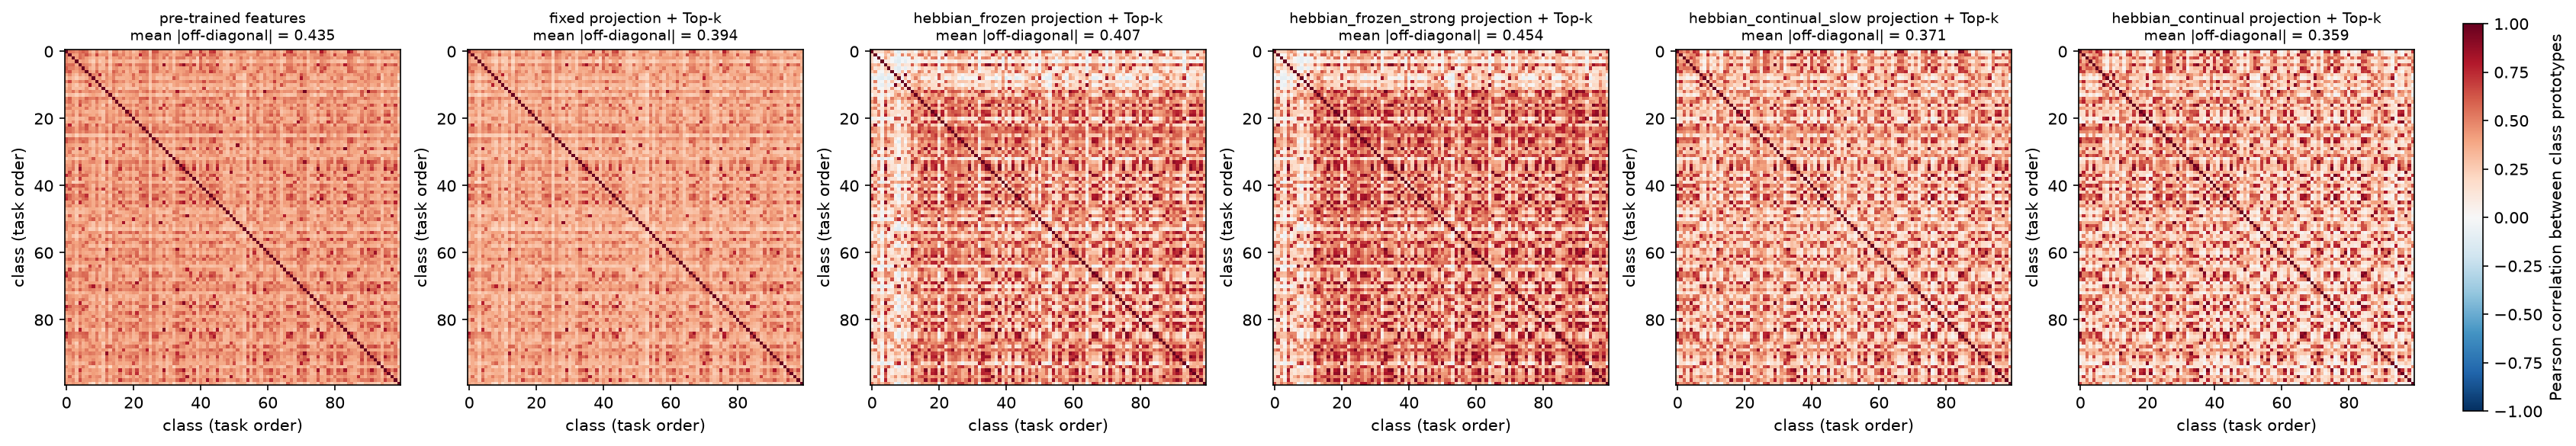
\includegraphics[width=\textwidth]{../results/analysis/prototype_correlation_seed1993.png}
\caption{Class-prototype correlation matrices before the projection (left) and after the sparse
projection + Top-$k$ for the fixed and the learned projections (seed 1993). Classes are ordered by
the task that introduces them; the first 10 are the classes the frozen Hebbian projection was
trained on.}
\label{fig:proto}
\end{figure}

\paragraph{Findings.}
\begin{itemize}
  \item The frozen Hebbian projection strongly decorrelates the classes it was trained on
        ($0.42 \to 0.15$) but makes the 90 classes of later tasks \emph{more} correlated than the
        random projection does ($0.395 \to 0.414$, and $\to 0.469$ with stronger learning). The
        units become tuned to the first task and lose the task-agnostic coverage of a random
        projection. Over all 100 classes the net effect is within seed noise for the weak setting
        and clearly worse for the strong one.
  \item The better decorrelation of first-task prototypes does not give better first-task accuracy
        (98.30 fixed vs 97.83 Hebbian right after task 1; 87.83 vs 87.33 at the end). The ridge
        solve already removes prototype correlation through $(G + \lambda I)^{-1}$, so decorrelating
        earlier is redundant.
  \item Continual updates are not viable with streaming statistics: $G$ and $Q$ of old tasks were
        accumulated under an older projection and cannot be recomputed without exemplars. Even a
        drift of 4\% in row direction (cosine 0.96, slow variant) costs 14 points of last accuracy
        and gives BWT $-24$; the default learning rate gives BWT $-77$. The \emph{final} continual
        projection decorrelates prototypes of all classes a little better than the random one
        (0.377 vs 0.395), so seeing all tasks helps the projection itself; it is the stale
        statistics that break.
  \item Cost: the Hebbian pass adds about 0.15\,s (0.4\,s for the strong setting) to the first task only.
\end{itemize}

\section{Task 2: Variance-Adaptive Generalized Ridge}

\paragraph{Method.} $\Lambda = \mathrm{diag}(\lambda_j)$ with
\[
\lambda_j = \lambda_{\mathrm{GCV}}\, s_j, \qquad
s_j = \left( \frac{G_{jj}}{\tfrac{1}{m}\sum_i G_{ii}} \right)^{\alpha},
\]
clamped to $[0.01, 100]$ and normalised to mean 1; $G_{jj}$ is the accumulated activity of
expanded dimension $j$. $G$, $Q$ and GCV are unchanged and the system $(G + \Lambda) W = Q$ is
solved by Cholesky.

\begin{table}[h]
\centering
\caption{Validation sweep over $\alpha$ (seed 1993; scalar ridge: 93.08 / 87.88).}
\label{tab:val2}
\small
\begin{tabular}{lcccccccc}
\toprule
$\alpha$ & $-2$ & $-1$ & $-0.5$ & $0.25$ & $0.5$ & $1$ & $2$ & $4$ \\
\midrule
Val avg  & 92.96 & 93.09 & 93.07 & 93.05 & 93.06 & 93.06 & 92.88 & 92.58 \\
Val last & 88.06 & 87.98 & 88.04 & 87.86 & 87.86 & 87.80 & 87.90 & 87.90 \\
\bottomrule
\end{tabular}
\end{table}

Accuracy is flat for $|\alpha| \le 1$. The final runs use $\alpha = 1$ (ridge on
variance-standardised dimensions, the principled choice) and $\alpha = -1$ (nominally best on
validation).

\paragraph{Which dimensions get the stronger ridge?} See Figure~\ref{fig:ridge}.
\begin{itemize}
  \item Activity is very uneven: $G_{jj}$ spans $6\times10^4$ to $1.3\times10^8$ (median
        $1.1\times10^7$), more than three orders of magnitude, because Top-$k$ keeps some units
        active for almost every image.
  \item Activity and correlation go together: the Spearman correlation between $G_{jj}$ and the
        correlation load of a dimension (mean absolute correlation with all other dimensions) is
        $0.989 \pm 0.0004$. With $\alpha = 1$, $\lambda_j$ therefore ranges from $10^4$ (lower
        clamp) to $9\times10^6$ around the scalar value $10^6$, and \textbf{the highly active
        dimensions, which are also the highly correlated ones, receive the stronger
        regularization} (Spearman of $\lambda_j$ with correlation load: 0.989).
\end{itemize}

\begin{figure}[h]
\centering
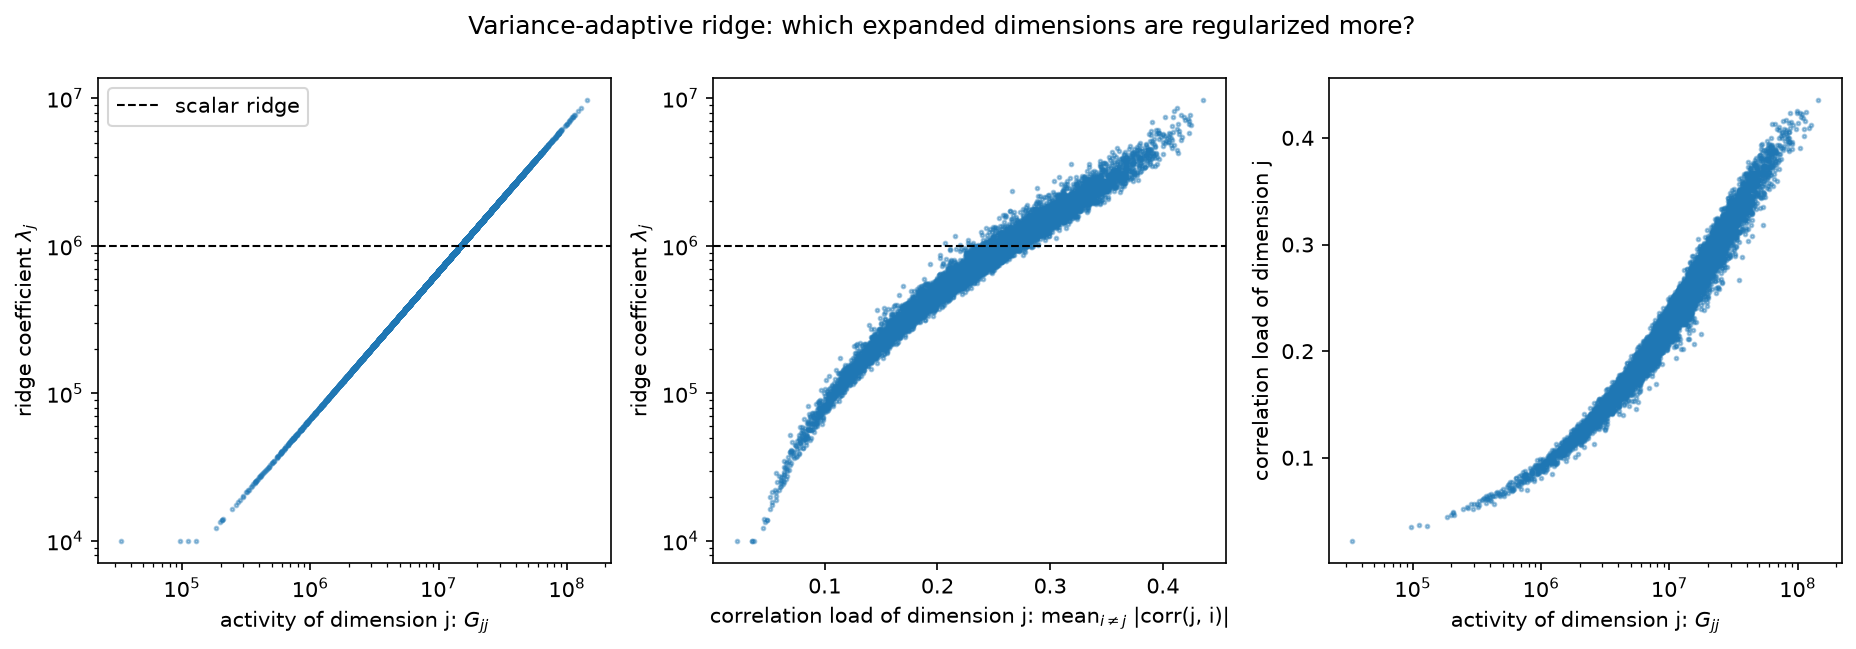
\includegraphics[width=\textwidth]{../results/analysis/adaptive_ridge_seed1993.png}
\caption{Variance-adaptive ridge with $\alpha = 1$ (seed 1993). Left: ridge coefficient against
activity $G_{jj}$. Middle: ridge coefficient against correlation load. Right: activity against
correlation load. The dashed line is the scalar ridge.}
\label{fig:ridge}
\end{figure}

\begin{table}[h]
\centering
\caption{Numerical conditioning of the final system $G + \Lambda$ (float64 eigenvalues, 3 seeds).}
\label{tab:cond}
\small
\begin{tabular}{lcc}
\toprule
Ridge & $\mathrm{cond}(G + \Lambda)$ & cond after diagonal (Jacobi) scaling \\
\midrule
scalar (original)       & $(5.3 \pm 0.07)\times10^4$ & $(1.8 \pm 0.1)\times10^5$ \\
adaptive, $\alpha = 1$  & $(1.05 \pm 0.34)\times10^6$ & $(3.6 \pm 0.01)\times10^4$ \\
adaptive, $\alpha = -1$ & $(9.8 \pm 0.3)\times10^4$ & $(4.5 \pm 0.3)\times10^5$ \\
\bottomrule
\end{tabular}
\end{table}

The plain condition number gets about $20\times$ worse with $\alpha = 1$, because weakly active
dimensions receive a much smaller ridge and the smallest eigenvalue drops. After symmetric
diagonal scaling, which is what determines the accuracy of a Cholesky solve, the $\alpha = 1$
system is about $5\times$ better conditioned than the scalar one. Neither effect is visible in
accuracy: all systems solve fine in float32.

\paragraph{Findings.} Accuracy, BWT and training time are unchanged within noise (paired $\Delta$
last acc $-0.01$ for $\alpha = 1$, $+0.06$ for $\alpha = -1$). Two reasons are consistent with the
data. First, GCV selects $10^6$, the lower edge of the grid, in every task of every run, so
regularization is already weak relative to the typical $G_{jj}$ ($10^7$) and redistributing it
across dimensions changes little. Second, with 10000 sparse dimensions the classifier is robust to
how the shrinkage is shared. Training time is the same because the solve is still one Cholesky
factorization.

\section{Outcome}

\begin{itemize}
  \item Both tasks are implemented as specified and evaluated on all requested metrics.
  \item Task 1: the stable (frozen) Hebbian projection costs 0.3 points of average and last
        accuracy; continual updates break the streaming statistics. The learned projection
        decorrelates only the classes it has seen.
  \item Task 2: the adaptive ridge matches the scalar ridge in accuracy, BWT and time; it gives
        stronger regularization to highly active, highly correlated dimensions and improves the
        diagonally scaled conditioning, while worsening the plain condition number.
  \item The original fixed random projection with scalar ridge remains the best configuration tested.
\end{itemize}

\section{Limitations}

\begin{itemize}
  \item One dataset (CIFAR-100) and one backbone; CUB-200-2011 and VTAB need a manual download and
        were not run.
  \item Three seeds. Effects below about 0.1 points should be read as ``no difference''.
  \item GCV always sits on the lower edge of the ridge grid given in \texttt{scripts/test\_cifar.sh};
        the original grid was kept on purpose, so the adaptive ridge was not tested with a wider grid.
  \item The explanation of why the frozen Hebbian projection does not help is supported by the
        first-task / later-task split in Table~\ref{tab:decor}, but was not tested with other
        learning rules (for example rules that explicitly decorrelate units).
\end{itemize}

\section{Reproduce}

\begin{verbatim}
source .venv/bin/activate
experiments/run_all.sh          # all test-set runs (about 50 min on an RTX 3070)
for s in 1993 1994 1995; do python experiments/analyze.py --seed $s; done
python experiments/summarize.py > results/summary.md
# validation sweep:
python experiments/make_val_cache.py cache/cifar100_vit_seed1993 \
       cache/cifar100_vit_seed1993_val
experiments/sweep_val.sh
\end{verbatim}

\end{document}
